\subsection*{}
Con el paso de los annos hemos visto en el procesado de los datos una oportunidad de oro, 
tanto para mejora nuestra vida diaria como para intentar predecir
eventos futuros. Por esta razon, surge la tendecia de almacenar todos los datos que tenemos 
a nuestro alrededor con la esperanza de que algun dia sean tratados.
Como por el momento no tienen ningun fin en concreto, se almacena competamente todo, sin discriminacion.
Sin saber si en algun momento seran utiles o no.
Por otra parte, multiples empresas tanto publicas como privadas, incluidas nuestros gobiernos, 
en su compromiso por la transparecia y esperanza de sacarle provecho, publican estos datos periodicamente.

Aunque estos datos esten disponibles publicamente, no significa que sean provechosos para el 
usuario medio, ya que se enfrenta a multiples retos.
\begin{itemize}
    \item Localizacion. Los datos se encuentran disponibles en portales de datos abiertos organizados 
    y estructurados, normalmente se necesita una tarea de busqueda y seleccion
    a veces complicada. Aunque las empresas ponen cada vez mas de su parte en ofrecer una interfaz 
    agradable y funcional a los usuarios, esta tarea requiere de un trabajo de investigacion por parte del usuario,
    ya que posiblemente, debera buscar en distintos portales.
    \item Accesibilidad. Los datos suelen estan disponibles a traves de una interfaz de programacion 
    de aplicaciones (API) no facilmente interpretable por el usuario medio. Normalmente cuenta con 
    un documento que describe cada uno de los campos y valores que se presentan en el documento y como utilizar la API.
    \item Interpretabilidad. Usualmente los datos estan representados en un formato para ser procesado por 
    algun software, por lo que su lectura resulta complicada por el usuario medio, en el mejor de los casos, 
    estaran representados en una tabla y aun asi, sera muy dificil de extraer informacion.
    \item Almacenamiento. Los datos publicados son los mas recientes, por lo que no hay manera de obtener 
    un historico de los datos si no son almacenados periodicamente. Una vez extraidos los datos, el usuario debera 
    contar con una infraestructura que le permita almacenar los datos.
    \item Automatizacion. Este proceso tiende a ser arduo, por lo que sera necesario automatizarlo, de otra 
    forma el esfuerzo requerido por el usuario para extraer la informacion no le compensara.
     
\end{itemize}

Por lo tanto, no podemos decir que estos datos sean accesibles de una forma util para el usuario medio. 


Recordemos que el objetivo principal del acceso a los datos, es obtener conocimiento. Hay que tener en cuenta 
que los datos por si solos, no tienen ningun valor, ya que carecen de sentido, una vez integrados en un contexto,
nos aportara informacion, y analizando esta informacion, se obtendra el conocimiento.\\


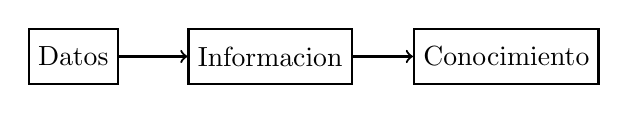
\begin{tikzpicture}[thick]
    \node[draw,rectangle,minimum size=20] (a) {Datos};
     \node[draw,rectangle,minimum size=20,right of= a, node distance=2.5cm] (b) {Informacion};
     \node[draw,rectangle,minimum size=20,right of=b, node distance=3cm] (c) {Conocimiento};
     \draw[->] (a) to (b);
    \draw[->] (b) to (c);
 
  \end{tikzpicture}
\\
Para poder obtener este valor de los datos, es necesario que el usuario interprete correctamente los datos, para
ello debe contar con conocimientos en la materia o realizar una tarea de investigacion, que le permita entender
los valores extraidos.

Ademas de entender cada campo y valor, el usuario debera serciorarse de que los datos cumplen las siguientes premisas:
\begin{itemize}
    \item Credibilidad. 
    \item Precision. 
    \item Consistencia.
    \item Interpretabilidad.
    \item Complitud.
\end{itemize}
--Ejemplos de las premisas--

--procesos ETL
--Base solida de diseno del sistema

, estos deberan ser analizados, 
discriminados y posiblemente habra que realizar diferentes calculos para poder obtener informacion util.

Asi pues, para que el usuario pueda obtener la informacion de una manera directa, requiere de conocimientos tanto debera
programacion como especificos de la materia y los recursos para crear una infraestructura que le permita implementar 
una representacion de los datos que le sea util.

--teoria sobre los datos sin procesamiento no son nada

--discriminacion de datos
--investigacion




----Respecto a polucion del aire 
Acudir a fuentes privadas
Instalacion de dispositivos
Ejemplos de bases de datos de distintas ciudades capitales
